\section{Random Dot Product Graphs}
\label{sec:ch5:rdpg}

Let's assume that you have $100$ people who live along a very long road that is $100$ miles long, and each person is $1$ mile apart. The nodes of your network represent the people who live along your assumed street, and the edges represent whether a given pair of people along the street are friends. However, there's a slight twist here: the people at the ends of the street are party hosts. If someone lives closer to one party host, they are going to tend to more frequently go to that host's parties than the other party host. Consequently, when someone lives near a party host, they are going to tend to be better friends with other people who go to that host's parties more frequently. How could you model such a situation?

Mathematically, for each person $i$, we could have a vector $\vec x_i$, that looks like this:
\begin{align*}
    \vec x_i &= \begin{bmatrix}
        \frac{100 - i}{100} & \frac{i}{100}
    \end{bmatrix}
\end{align*}

We could model the probability of two people $i$ and $j$ being friends with $\vec x_i^\top \vec x_j$, the inner product. Remember that this quantity is just the element-wise sum of the elements of each vector; that is:
\begin{align*}
    \vec x_i^\top \vec x_j = \sum_{u = 1}^d x_{id}y_{jd}
\end{align*}

For instance, $\vec x_1 = \begin{bmatrix}1 \\ 0\end{bmatrix}$, and $\vec x_{100} = \begin{bmatrix} 0 \\ 1\end{bmatrix}$. Note that:
\begin{align*}
p_{1,100} = \vec x_1^\top \vec x_j = 1 \cdot 0 + 0 \cdot 1 = 0
\end{align*}
What happens in between?

Let's consider another person, person $30$. Note that person $30$ lives closer to person $1$ than to person $100$.  Here, $\vec x_{30} = \begin{bmatrix} \frac{7}{10}\\ \frac{3}{10}\end{bmatrix}$. This gives you that:
\begin{align*}
p_{1,30} &= \vec x_1^\top \vec x_{30} = \frac{7}{10}\cdot 1 + 0 \cdot \frac{3}{10} = \frac{7}{10} \\
p_{30, 100} &= \vec x_{30}^\top x_{100} = \frac{7}{10} \cdot 0 + \frac{3}{10} \cdot 1 = \frac{3}{10}
\end{align*}
So this means that person $1$ and person $30$ have a $70\%$ probability of being friends, but person $30$ and $100$ have only a $30\%$ probability of being friends.

This feels like it might work out for us, so let's formalize it a little bit. We will do this with the Random Dot Product Graph (RDPG). This concept was first introduced by \cite{Young2007}. With the RDPG, you can have random networks which are much more complex than those you saw with the $ER_n(p)$ and the $SBM_n(\vec z, B)$ random networks, but {still} have a discernable structure to them.

% \subsection{Defining the RDPG}

\subsection{The latent position matrix}

We parameterize the RDPG using a matrix $X$ called the \textit{latent position matrix}. Each row $\vec x_i$ will be called the \textit{latent position of the node} $i$. In matrix form, $X$ looks like this:

\begin{align*}
 X = \begin{bmatrix}
     \vdash & \vec x_1^\top & \dashv \\
     \vdash & \vec x_2^\top & \dashv \\
     & \vdots & \\
     \vdash & \vec x_n^\top & \dashv
 \end{bmatrix}
\end{align*}

We will call the columns of $X$ the \textit{latent dimensions}, and the total number of columns that $X$ has will be called the \textit{latent dimensionality}. We will often use the letter $d$ to denote the latent dimensionality of the latent position matrix $X$. For this reason, we say that $X$ is an $n$ row (one for each node) and $d$ column (one for each latent dimension) matrix, written as $X \in \mathcal{R}^{n \times d}$. Therefore, the latent position of the node $i$, $\vec x_i$, is a $d$-dimensional vector. 


\subsection{Conceptualizing the RDPG}

We call this model the RDPG because the probabilities of edges existing are based on {dot products} between pairs of latent positions for the different nodes in the network. The way that you can think of the RDPG random network is that the edges depend on a latent position matrix $X$. For each pair of nodes $i$ and $j$, you have a unique coin (we will call this the $(i,j)$ coin) which has a $\vec x_i^\top \vec x_j$ chance of landing on heads, and a $1 - \vec x_i^\top \vec x_j$ chance of landing on tails. If the $(i,j)$ coin lands on heads, the edge between nodes $i$ and $j$ exists, and if the $(i,j)$ coin lands on tails, the edge between nodes $i$ and $j$ does not exist. As before, this coin flip is performed independent of the coin flips for all of the other edges. If $\mathbf A$ is a random network which is $RDPG$ with a latent position matrix $X$, we say that $\mathbf A$ is an $RDPG_n(X)$ random network. 

\subsection{How do you simulate samples of $RDPG_n(X)$ random networks?}


The procedure in Algorithm \ref{alg:ch5:rdpg} will produce for you a network $A$, which has nodes and edges, where the underlying random network $\mathbf A$ is an RDPG random network. 

\begin{algorithm}[h]\caption{Simulating a sample from an $SBM_n(\vec z, B)$ random network}
\label{alg:ch5:rdpg}
\SetAlgoLined
\KwData{$n$ a number of nodes\newline $\vec X$ a latent position matrix whose rows indicate the $d$-dimensional latent position vectors for each node}
\KwResult{The adjacency matrix of a sample from the random network.}
\For{$i$ in $1$:$n$} {
    \For{$j > i$}{
        Obtain a weighted coin $(i,j)$ which has a probability of $\vec x_i^\top \vec x_j$ of landing on heads, and a $1 - \vec x_i^\top \vec x_j$ probability of landing on tails.

        Flip the $(i,j)$ coin, and if it lands on heads, the corresponding entry $a_{ij}$ in the adjacency matrix is $1$. If the coin lands on tails, the corresponding entry $a_{ij} = 0$.

        Let $a_{ji} = a_{ij}$.
    }
}

\end{algorithm}

Let's return to the party example we started above. The first thing that we need to worry about is deciphering what our latent position matrix looks like. Let's code it up below:

\begin{lstlisting}[style=python]
import numpy as np
from graphbook_code import lpm_heatmap

n = 100  # the number of nodes in your network
# design the latent position matrix X according to 
# the rules we laid out previously
X = np.zeros((n,2))
for i in range(0, n):
    X[i,:] = [(n - i)/n, i/n]

lpm_heatmap(X, ytitle="Person", xticks=[0.5, 1.5], xticklabels=[1, 2],
                xtitle="Latent Dimension", title="Latent Position Matrix, X")
\end{lstlisting}

This latent position matrix is shown in Figure \ref{fig:ch5:rdpg}(A). Next, we can use graspologic with this latent position matrix to sample an $RDPG_n(X)$ random network:

\begin{lstlisting}[style=python]
from graspologic.simulations import rdpg
from graphbook_code import heatmap

# sample an RDPG with the latent position matrix
# created above
A = rdpg(X, loops=False, directed=False)

# and plot it
heatmap(A.astype(int), xtitle="Person", ytitle="Person",
          title="$RDPG_{100}(X)$ Simulation")
\end{lstlisting}

A sample from the $RDPG_n(X)$ random network is shown in Figure \ref{fig:ch5:rdpg}(B).

\begin{figure}[h]
    \centering
    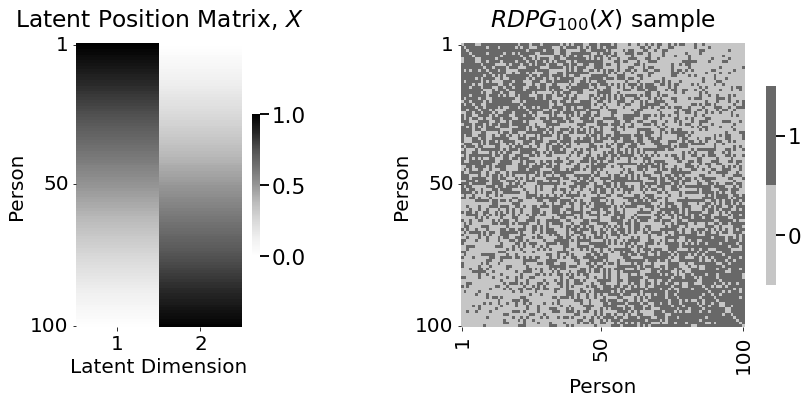
\includegraphics[width=\linewidth]{representations/ch5/Images/rdpg.png}
    \caption[Visualizing the Random Dot Product Graph]{\textbf{(A)} the latent position matrix. \textbf{(B)} a sample of an $RDPG_n(X)$ random network.}
    \label{fig:ch5:rdpg}
\end{figure}

\subsection{$RDPG_n(X)$ random networks generalizes to a broad class of problems}

In certain situations, the $RDPG_n(X)$ model can generalize the $SBM_n(\vec z, B)$ model that we learned about in Section \ref{sec:ch5:sbm}. The particular situation that the $RDPG_n(X)$ model is extremely effective for is known as {homophily} \cite{Hoff2007Dec,Athreya2017Jan}. Homophily exists in a network when the relationship between nodes which have similar characteristics (such as the same community assignment) are stronger than the relationships between nodes which have different characteristics (such as a pair of nodes with different community assignments). 

In the example that we covered in Section \ref{sec:ch5:sbm}, this is analogous to the idea that students from the same school were more likely to be friends than students from different schools. This is an extremely powerful concept, since many networks (and many network machine learning questions) that we will learn to ask will center around this concept of homophily.

To better understand when an $RDPG_n(X)$ random network will generalize an $SBM_n(\vec z, B)$ random network, we first will turn to the most generalizable independent-edge random network model: the Inhomogeneous Erd\"os R\'enyi Random Networks.

\subsection{Read on for more}

If you want a deeper level of technical depth on Random Dot Product Graphs, please see Appendix \ref{app:ch12:rdpg}.


\newpage